\documentclass[tikz,border=8pt]{standalone}
\usepackage{tikz}
\usetikzlibrary{arrows.meta}
\usepackage[T1]{fontenc}
\usepackage[semibold]{ebgaramond}   % EB Garamond, semibold as \bfseries

% --- Theme palette (from theme.md) ---
\definecolor{primary}{HTML}{6B4FA0}     % Lavender Purple  — DB, × gate, dots
\definecolor{accent}{HTML}{E8B84B}      % Golden Yellow    — probability, "SQL"
\definecolor{highlight}{HTML}{C4664A}   % Warm Terracotta  — + gates
\definecolor{textprimary}{HTML}{2A1850} % Deep Plum        — "Prov"
\definecolor{muted}{HTML}{8A7A9B}       % Dusty Mauve      — wires

\tikzset{
  gate/.style={circle, draw=#1, fill=#1!15, thick,
    inner sep=3pt, font=\bfseries, text=#1},
  wire/.style={semithick, muted!80, -{Stealth[length=2.5pt,width=2pt]}}
}

\begin{document}
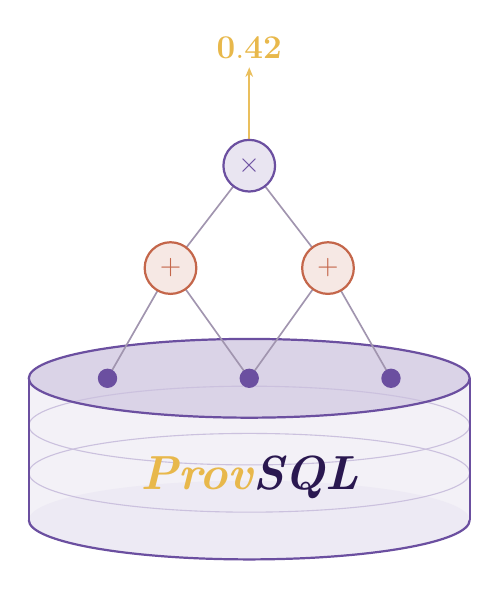
\begin{tikzpicture}

\def\CW{2.8}    % cylinder half-width
\def\CH{1.8}    % cylinder body height
\def\CER{0.5}   % ellipse minor radius (perspective)
\pgfmathsetmacro{\discOne}{\CH/3}
\pgfmathsetmacro{\discTwo}{2*\CH/3}
\pgfmathsetmacro{\baseY}{\CH}          % circuit starts at center of top ellipse
\pgfmathsetmacro{\pY}{\baseY+1.4}
\pgfmathsetmacro{\xY}{\baseY+2.7}
\pgfmathsetmacro{\probY}{\baseY+4.2}

%--- Database cylinder ---

\fill[primary!8]  (-\CW,0)  rectangle (\CW,\CH);
\fill[primary!12] (0,0)      ellipse (\CW cm and \CER cm);
\fill[primary!25] (0,\CH)    ellipse (\CW cm and \CER cm);

% Stacked-disc lines
\draw[primary!35, thin] (0,\discOne) ellipse (\CW cm and \CER cm);
\draw[primary!35, thin] (0,\discTwo) ellipse (\CW cm and \CER cm);

% ProvSQL wordmark — two overlapping nodes with \phantom for correct centering,
% avoids Inkscape misrendering \textcolor splits within a single node.
\node[font=\LARGE\bfseries\itshape, text=textprimary] at (0, \CH*0.3) {\phantom{Prov}SQL};
\node[font=\LARGE\bfseries\itshape, text=accent]       at (0, \CH*0.3) {Prov\phantom{SQL}};

% Cylinder outline
\draw[primary, thick] (-\CW,0) -- (-\CW,\CH);
\draw[primary, thick] ( \CW,0) -- ( \CW,\CH);
\draw[primary, thick] (0,\CH)   ellipse (\CW cm and \CER cm);
\draw[primary, thick] (-\CW,0)  arc(180:360:\CW cm and \CER cm);

%--- Provenance circuit ---

% 1. Wires first (under dots and gates)
\draw[wire] (-1.8,\baseY) -- (-1.0,\pY);
\draw[wire] (   0,\baseY) -- (-1.0,\pY);
\draw[wire] (   0,\baseY) -- ( 1.0,\pY);
\draw[wire] ( 1.8,\baseY) -- ( 1.0,\pY);
\draw[wire] (-1.0,\pY)    -- (0,\xY);
\draw[wire] ( 1.0,\pY)    -- (0,\xY);
\draw[accent!90, thick, -{Stealth[length=3.5pt,width=2.8pt]}]
  (0,\xY) -- (0,\probY-0.25);

% 2. Dots
\foreach \x in {-1.8, 0, 1.8} {
  \fill[primary] (\x,\baseY) circle (3.5pt);
}

% 3. Gates
\node[gate=highlight] at (-1.0,\pY) {$+$};
\node[gate=highlight] at ( 1.0,\pY) {$+$};
\node[gate=primary]   at (   0,\xY) {$\times$};

% 4. Probability — accent gold, EB Garamond semibold italic (theme: stat = EB Garamond 600 italic, gold)
\node[font=\large\bfseries\itshape, text=accent] at (0,\probY) {$\mathbf{0.42}$};

\end{tikzpicture}
\end{document}
